%% Copyright 1998 Pepe Kubon
%%
%% `two.tex' --- 2nd chapter for thes-full.tex, thes-short-tex from
%%               the `csthesis' bundle
%%
%% You are allowed to distribute this file together with all files
%% mentioned in READ.ME.
%%
%% You are not allowed to modify its contents.
%%

%%%%%%%%%%%%%%%%%%%%%%%%%%%%%%%%%%%%%%%%%%%%%%%%%
%
%     Chapter 2   
%
%%%%%%%%%%%%%%%%%%%%%%%%%%%%%%%%%%%%%%%%%%%%%%%%

\chapter{Word Embeddings}
\label{wordvizChapter}

\section{What are word embeddings?}\label{intro-biembedding}
Semantic relations between words denote how two words are related or how close their meanings are. One way to represent this relation is by representing each word as a vector (also called word embeddings) such that, words which are similar, their vectors would lie closer to each other in some $n$ dimension space. Whereas, vectors of dissimilar words would lie far apart. When creating the word embeddings, we assume that words are characterized by the words that surround it, that is the company that the word keeps \cite{Harris1954}. The relation between two vectors (words) is represented by using a displacement vector, that is, a vector between two vectors. The displacement vector can help us find relations like $queen : king :: woman : man$, which would mathematically be denoted as $v_{queen} - v_{king} = v_{woman} - v_{man}$. Here, $v_{i}$ means an $n$-dimension vector of the word $i$. 

Learning word embeddings broadly falls into two categories. \textit{Clustering  based representations}, often use hierarchical clustering methods to group similar words based on their contexts. Brown Clustering \cite{Brown1992} and \cite{Pereira1993} are the two most dominant approaches. Hidden Markov Models can also be used to induce clustering on words \cite{Huang2009}. The problem with clustering approach is that the representations generated are sparse vectors. The reason they are sparse is because the vectors generated would generally be one-hot vectors. Such vectors are contains binary values 0 or 1 where 1 indicates the cluster number to which the word belongs. To reduce the sparsity issues, the other approach is to generate \textit{dense representations} of words. These representations are low dimensional real valued dense vectors. These embeddings can be generated by using latent semantic analysis \cite{Deerwester1990}, canonical correlation analysis \cite{Dhillon2011}, neural-networks \cite{Collobert2008, Huang2012, Mikolov2013a, Mikolov2013b}.

As estimating Bi-LMs required parallel corpora of two languages, it is natural to utilize bilingual word embeddings that denote semantic relations among words across two languages, that is words which are semantically similar in either of the languages are close to each other in some $n$-dimension space. This enables us to understand how close a word in one language would be to another word in the second language. For example, the English word \textit{lake} and Chinese word \textzh{潭} \textit{(deep pond)}, even though they are not direct translations of each other, but due to their semantic similarity, they would be close to each other in some $n$-dimension space. And words which are semantically similar to \textzh{潭} \textit{(deep pond)} and possibly direct translations of \textit{lake} would also be close to each other in that $n$-dimension space. For word embeddings, we measure semantic similarity by measuring the cosine similarity between two word embeddings. It is formally defined as:
\begin{eqnarray}
similarity = cos(\theta) = \frac{\textbf{A}.\textbf{B}}{||\textbf{A}|| ||\textbf{B}||} = \frac{\sum_{i=1}^{n}A_iB_i}{\sqrt{\sum_{i=1}^{n}A_i^2} \sqrt{\sum_{i=1}^{n}B_i^2}}
\end{eqnarray}

Here, $\textbf{A}$ and $\textbf{B}$ are two vectors of size $n$.

Bilingual word embeddings have been created by using various techniques like latent dirichlet allocation and latent semantic analysis \cite{BoydGraber2012, Zhao2006}, canonical correlation analysis \cite{Faruqui2014}, neural-networks \cite{Klementiev12, Zou13, Mikolov2013c, Hermann14, Chandar2014}. In the next section we discuss the reasons for choosing the algorithms to create monolingual and bilingual word embeddings.

\section{Creating Word Embeddings}
As stated in Section~\ref{intro-biembedding}, the underlying idea of most of the methods is based on the concept that the meaning of a word can be determined by the \textit{company that it keeps}. This idea is the underlying method for most of the work done to create monolingual and bilingual word embeddings. For both the embeddings, most of the popular approaches are based on using either canonical correlation analysis~\cite{Dhillon2011, Faruqui2014} and neural networks~\cite{Collobert2008, Huang2012, Klementiev12, Mikolov2013a, Mikolov2013b, Mikolov2013c, Zou13, Hermann14, Chandar2014}. Neural network approaches to create word embeddings have been widely adopted due to the following advantages:
\begin{itemize}
	\item Training the networks can be done using parallel processing and distributed processing.
	\item Graphical processing units (GPU) can be utilized for faster training.
	\item If new data is available for training, the weights of the network can be updated by only using the new data and not the previously used training data. That is, the network does not need to be retrained by using all the previous and new training data. Matrix factorization methods like canonical correlation analysis and latent semantic analysis would require retraining of models using all the data.
	\item They are currently state of the art methods in producing good quality word embeddings.
\end{itemize}

Due to their speed of training and being the state of the art algorithms for training embeddings, we decided to use neural network based approach. For creating monolingual word embeddings we utilize \textbf{Word2Vec}~\cite{Mikolov2013a,Mikolov2013b,Mikolov2013c}, as it is currently state of the art toolkit for creating monolingual word embeddings. We will explain the usage of monolingual embeddings in Chapter~\ref{two}. 

For creating bilingual word embeddings, \cite{Zou13} utilize sentence aligned parallel corpora and their alignments to induce the embeddings whereas \cite{Hermann14} only utilizes a sentence aligned parallel corpora (they state that there is no theoretical dependence on sentence aligned parallel corpora and technically it could also be used with document aligned parallel corpora). As creating alignments is not perfect and they have a small margin of error (the state of the art method to create alignments~\cite{Kirkpatrick2010} for Chinese>English parallel corpus has an alignment error rate of 30\%), using word embeddings that require alignments~\cite{Zou13} would increase the chances of propagating errors. Hence, to keep the possibility of errors in creating alignments and creating bilingual word embedding independent of each other, we use the work of \cite{Hermann14} to create the bilingual word embeddings.

When bilingual word embeddings we need to manually choose multiple hyper-parameters for the algorithms. Varying the hyper-parameters changes the embeddings that are generated. To understand the effects of the hyper-parameters and to choose the ones which give good embeddings we introduce \textbf{WordEmbeddingsViz}\footnote{WordEmbeddingsViz: Tool to visualize bilingual word embeddings \url{https://github.com/anoopsarkar/WordEmbeddingsViz}}, a tool to visualize bilingual word embeddings and to study the effects of different values of hyper-parameters.

In the next section we explain how one can use WordEmbeddingsViz to choose the best embedding parameters.

\section{Visualizing Word Embeddings} \label{WordEmbeddingsViz}

\textbf{WordEmbeddingsViz} enables a user to visualize bilingual word embeddings. The tool uses t-Distributed Stochastic Neighbor Embedding (t-SNE)~\cite{tSNE} to project the embeddings into two dimension space. t-SNE is a non linear dimensionality reduction technique. t-SNE constructs a probability distribution over pairs of objects in high dimension such that similar objects (that is, objects which are close to each other) have a high probability whereas dissimilar objects (objects that are far apart) have a low probability. t-SNE defines a similar probability distribution over pairs of objects in lower dimension and minimizes the Kullback-Leibler divergence between the two distributions. In the higher dimension space, it uses Gaussian distribution to measure the similarity between objects, whereas in lower dimension space, it uses a Student's t-distribution to measure the similarity. This is because, Student's t-distribution has a long tail and it allows dissimilar objects to be modeled far apart.

To use visualize the embeddings, a user will upload the following for each language:
\begin{itemize}
	\item Word Embeddings
	\item Words
	\item Training Corpus (with part-of-speech for one language)
	\item Alignments (optional)
\end{itemize}

\begin{figure}[htbp]
	\begin{center}
		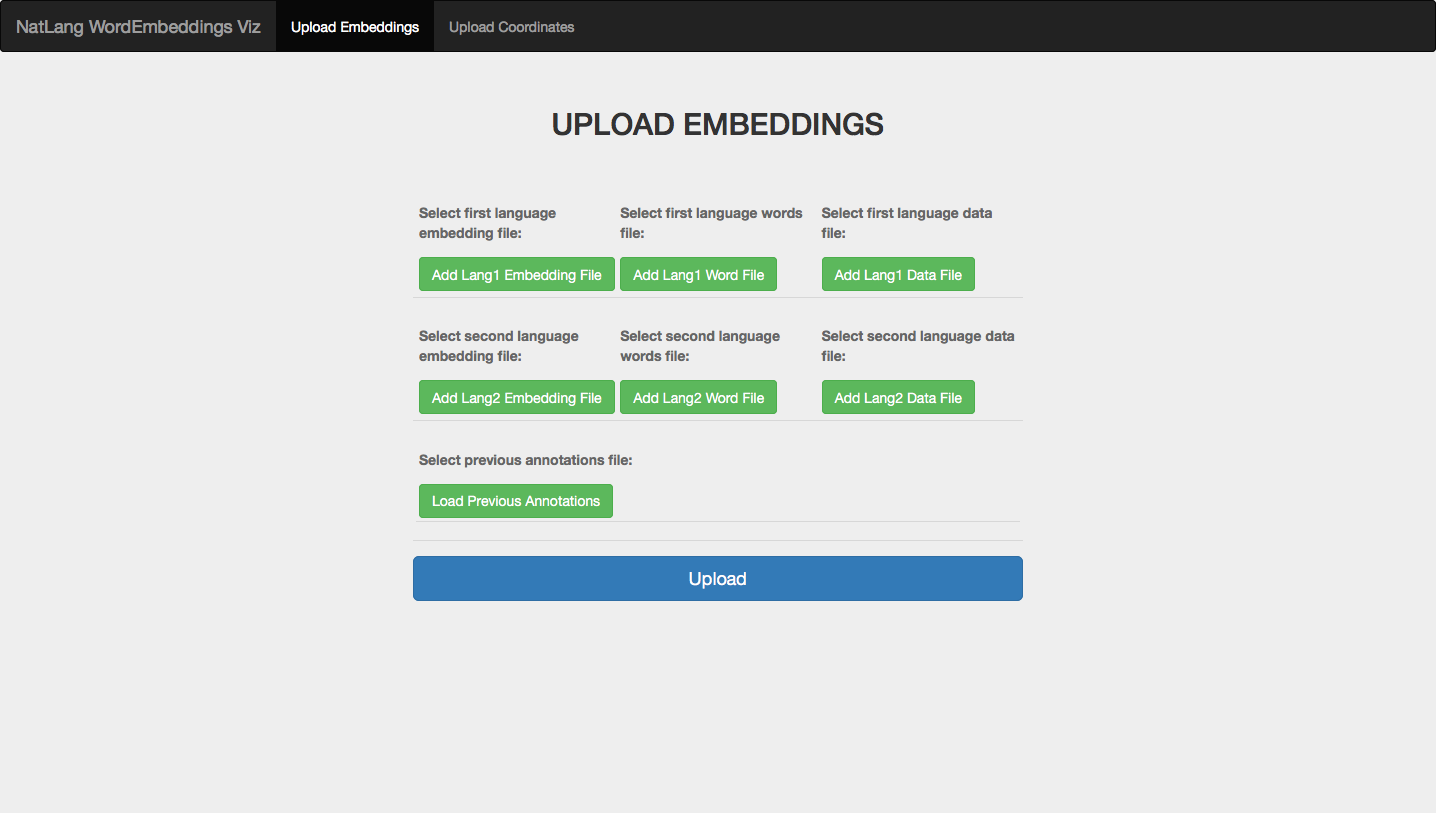
\includegraphics[width=\textwidth]{files/images/viz1}
	\end{center}
	\caption{WordEmbeddingsViz upload screen: Here, the user can upload bilingual word embeddings, word list, training corpus and alignments (optional)}
	\label{fig:viz1}
\end{figure}

Figure~\ref{fig:viz1} shows the upload screen where a user can upload the required data.

We require part-of-speech(POS) for one of the languages as this will be used by the tool to show a list of top 1000 words by their occurance count for \textit{verb, noun, adjective \& adverb} POS tags. For our work, we extracted POS tags for English data using Stanford POS tagger~\cite{POS}.

\textbf{WordEmbeddingsViz} will perform non-linear dimensionality reduction using \textbf{tSNE} on the word embeddings. The dimensions would be reduced to two dimensions. The value of these dimensions for each word would be treated as \textit{x} and \textit{y} coordinates to visualize them as a scatter plot. Figure~\ref{fig:viz2} shows the scatter plot for bilingual word embeddings of Chinese(Zh)-English(En) parallel corpus. The user can then zoom into the scatter plot to look at the word embeddings. The user can also select one of the English words from the sidebar (sidebar shows a list of top 1000 for each of the verbs, nouns, adjectives and adverbs). On selection of a word from the sidebar, that word will be highlighted and the user can then zoom in to look at the neighbouring embeddings. If for any English word, there one or more Chinese words in the neighbourhood that are possible translation of that English word, then the user can align them using the alignment option built into the tool. Figure~\ref{fig:viz3} and Figure~\ref{fig:viz4} shows examples of alignments between English words \textit{broadcast, braodcast \& broadcasting, and, clocks, timepiece \& chiming} along with their Chinese counterparts. The alignments can also be downloaded which can then be utilized for various usecases, such as, using the annotated alignments as information in word alignment algorithms.

\begin{figure}[htbp]
	\begin{center}
		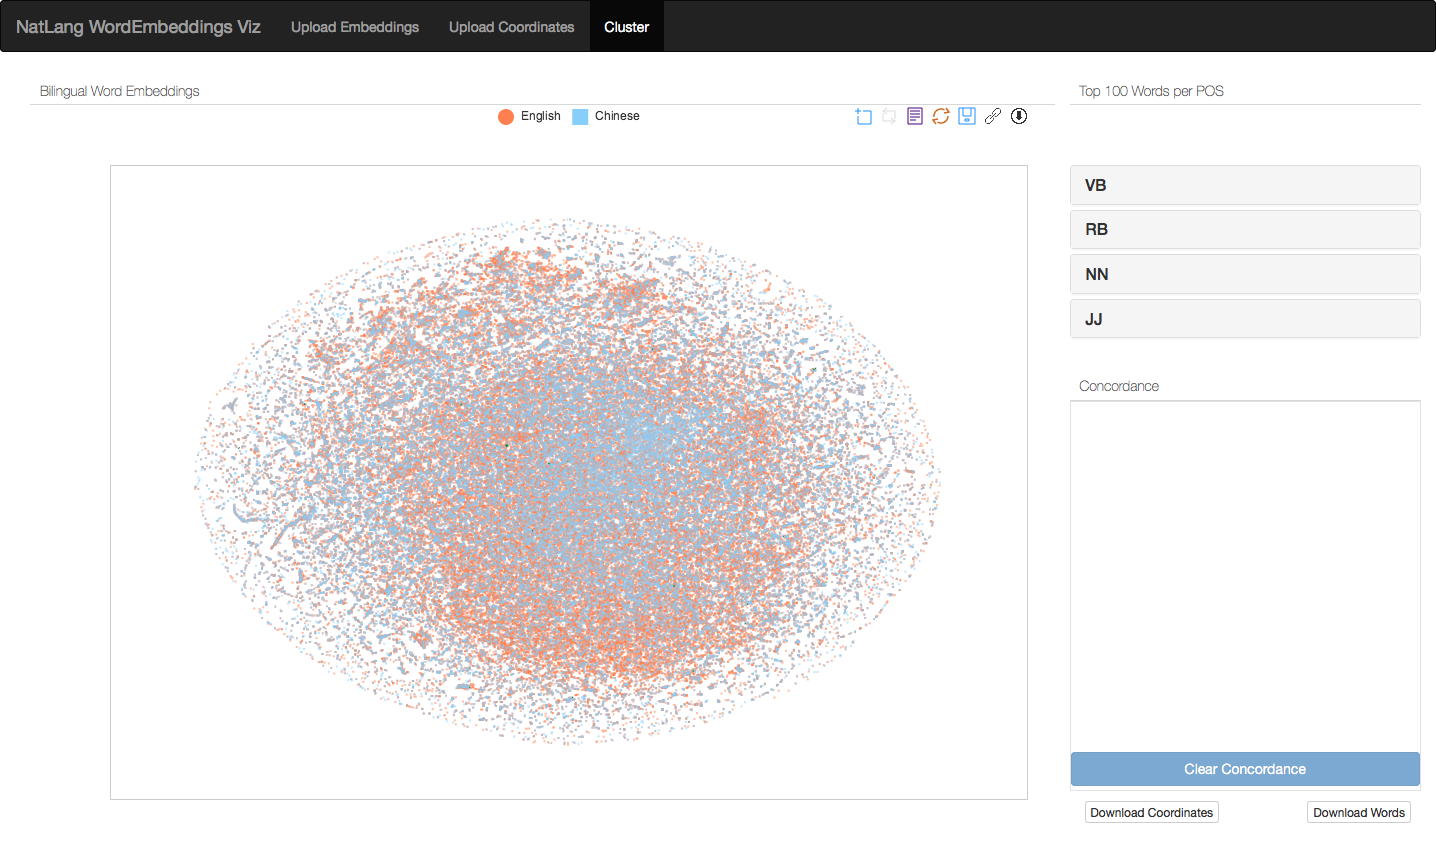
\includegraphics[width=\textwidth]{files/images/viz7}
	\end{center}
	\caption{WordEmbeddingsViz: A scatter plot of word embeddings of Zh-En parallel corpus. Orange squares represent English words and blue circles represent Chinese words.}
	\label{fig:viz2}
\end{figure}

\begin{figure}[htbp]
	\begin{center}
		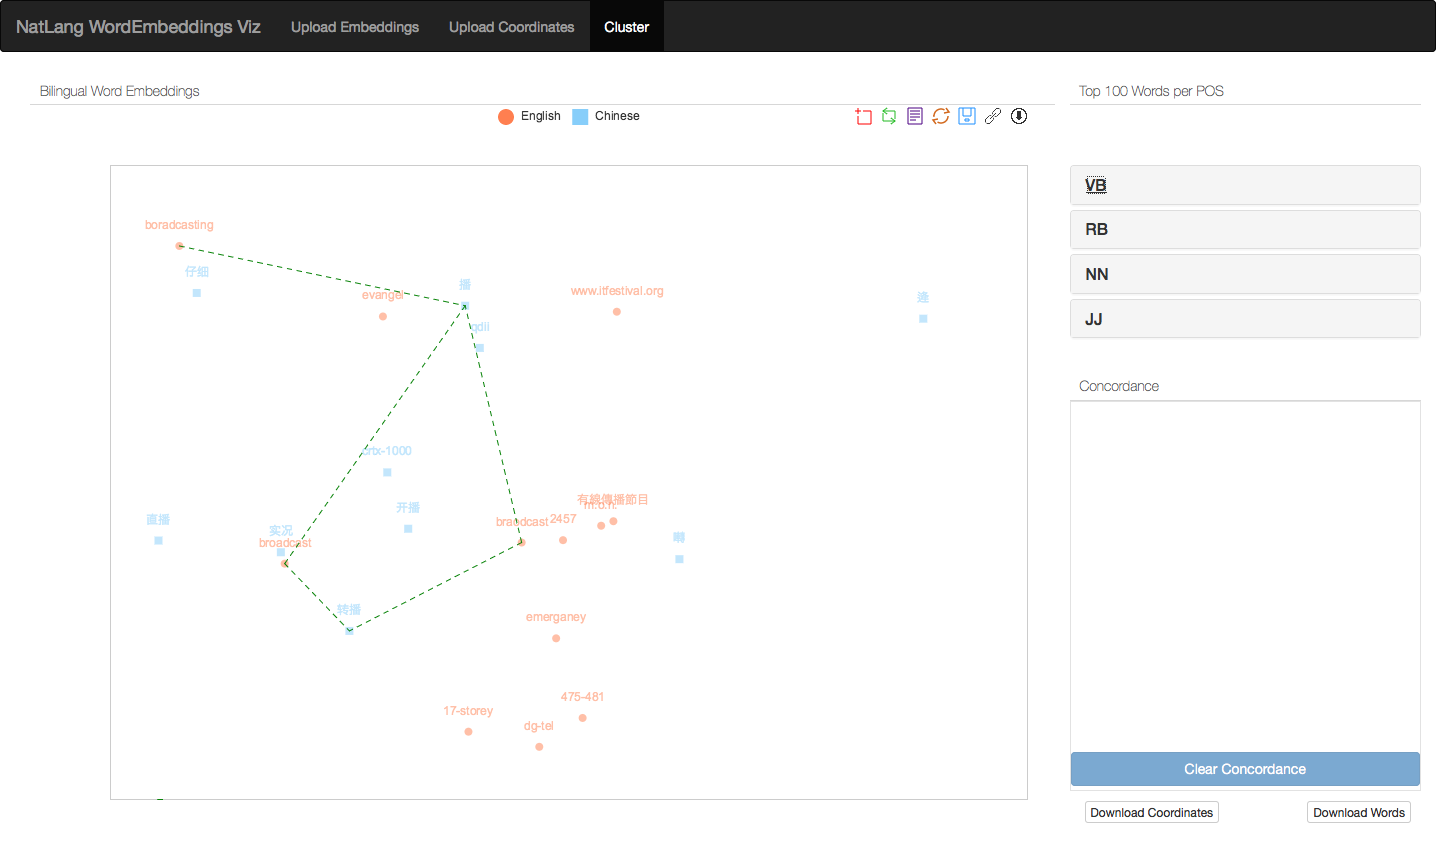
\includegraphics[width=\textwidth]{files/images/viz6}
	\end{center}
	\caption{WordEmbeddingsViz: Alignments of English words \textit{broadcast, braodcast, broadcasting} with their Chinese counterparts.}
	\label{fig:viz3}
\end{figure}

\begin{figure}[htbp]
	\begin{center}
		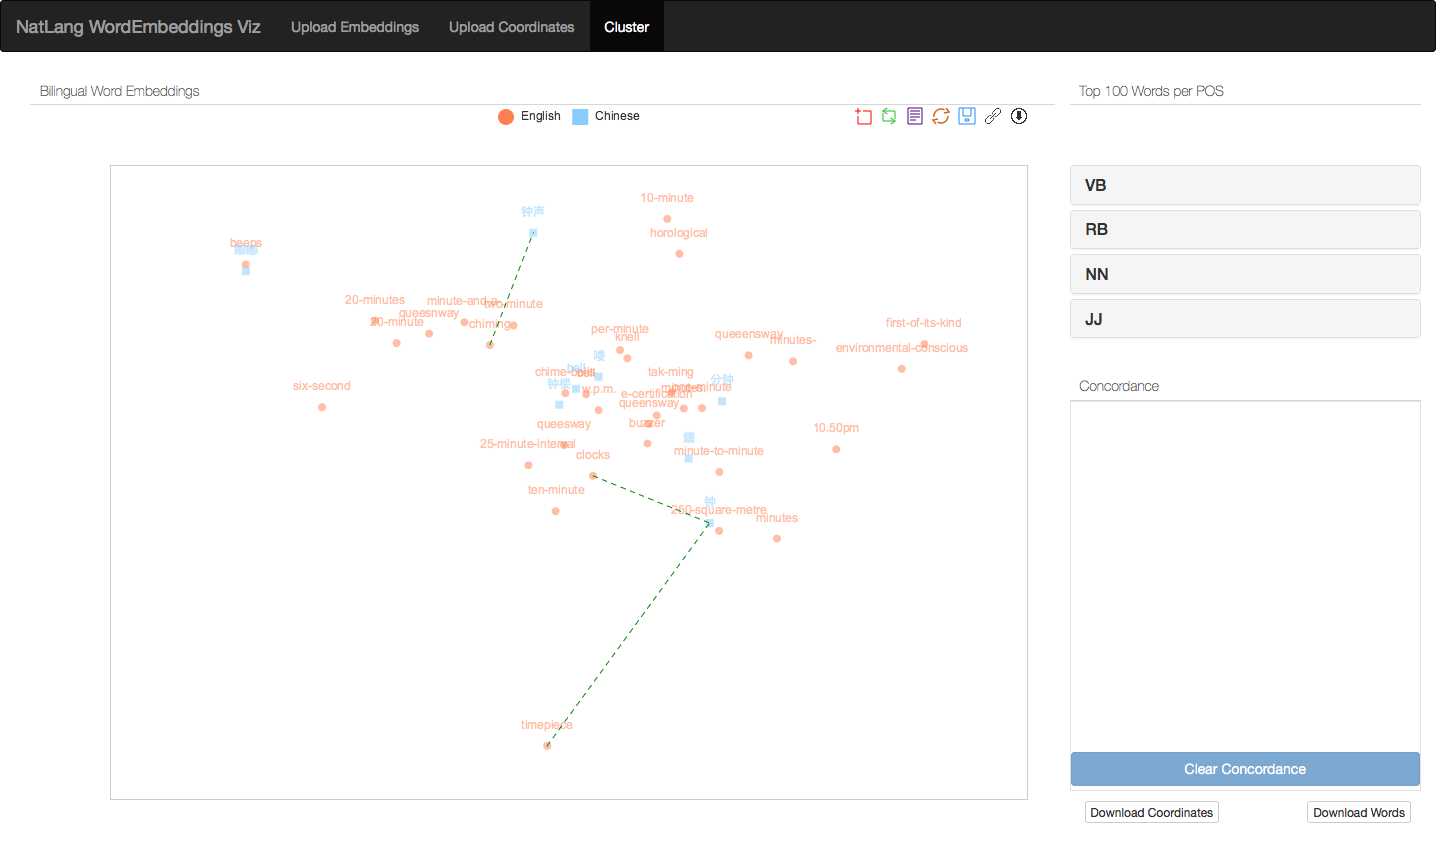
\includegraphics[width=\textwidth]{files/images/viz4}
	\end{center}
	\caption{WordEmbeddingsViz: Alignments of English words \textit{clocks, timepiece \& chiming} with their Chinese counterparts.}
	\label{fig:viz4}
\end{figure}

Using \textbf{WordEmbeddingsViz}, a human annotator can look at bilingual word embeddings generated with different parameters. If the embeddings generated are of good quality then semantically similar words in two languages would lie close to each other in the projected space.

\section{Summary}
In this chapter we introduced word embeddings and bilingual word embeddings. We also release a tool \textbf{WordEmbeddingsViz}, which we developed to judge the bilingual word embeddings. In the next chapter, we will provide an in depth description of bilingual language models and our approach of using word embeddings to model bilingual language models.